\section{Modelagem Funcional e Comportamental}
\label{sec:4.2}

A modelagem funcional tem como objetivo descrever as interações entre os usuários e o sistema, delimitando o escopo das funcionalidades e o comportamento esperado frente a diferentes cenários de uso. Segundo \citeonline{pressman2016}, essa etapa é fundamental para validar se os requisitos levantados correspondem às expectativas dos stakeholders, servindo como guia visual e textual para o desenvolvimento.

\subsection{Atores do Sistema}
\label{subsec:4.2.1}

O sistema IGRIS é composto por cinco atores, cada um com responsabilidades bem delimitadas conforme ilustrado no Diagrama de Casos de Uso.

O usuário representa o ator base do sistema. Todo acesso ao IGRIS é autenticado, cabendo ao usuário as operações comuns: autenticar-se, selecionar ou trocar de perfil, recuperar senha, realizar cadastro via link de convite e enviar feedback.

O coordenador é o ator gestor do fluxo acadêmico. Suas responsabilidades abrangem manter a disponibilidade dos professores, gerenciar disciplinas, turmas, cursos e matrizes, vincular disciplinas a cursos, manter turnos e dias letivos, gerar o link de cadastro de professores, além de gerar, salvar e visualizar a grade horária.

O professor alimenta o sistema com suas próprias informações: mantém sua disponibilidade de horários, registra as disciplinas que leciona e visualiza a própria grade gerada.

A instituição é responsável por operações de gestão de coordenadores: manter coordenadores e coordenações vinculadas à instituição.

O administrador do sistema possui acesso privilegiado: concede ou revoga perfis de acesso, mantém configurações globais do sistema, gerencia instituições e usuários, visualiza feedbacks e mantém as configurações de geração de grade, incluindo os parâmetros matemáticos dos microsserviços.

\subsection{Diagrama de Casos de Uso}
\label{subsec:4.2.2}

O Diagrama de Casos de Uso do IGRIS representa graficamente todas as interações possíveis entre os cinco atores do sistema e suas respectivas funcionalidades, organizadas por perfil de acesso e nível de responsabilidade. O diagrama consolida em uma única visão as operações de cada ator: desde as funcionalidades comuns ao Usuário (autenticação, seleção de perfil, feedback), passando pelas responsabilidades do Coordenador (gestão acadêmica completa e geração de grade), do Professor (disponibilidade e disciplinas lecionadas), da Instituição (gestão de coordenação) e do Administrador do Sistema (configuração e controle de acesso).

\begin{figure}[p]
\centering
\caption{Diagrama de Casos de Uso do IGRIS}
\label{fig:casos_de_uso}
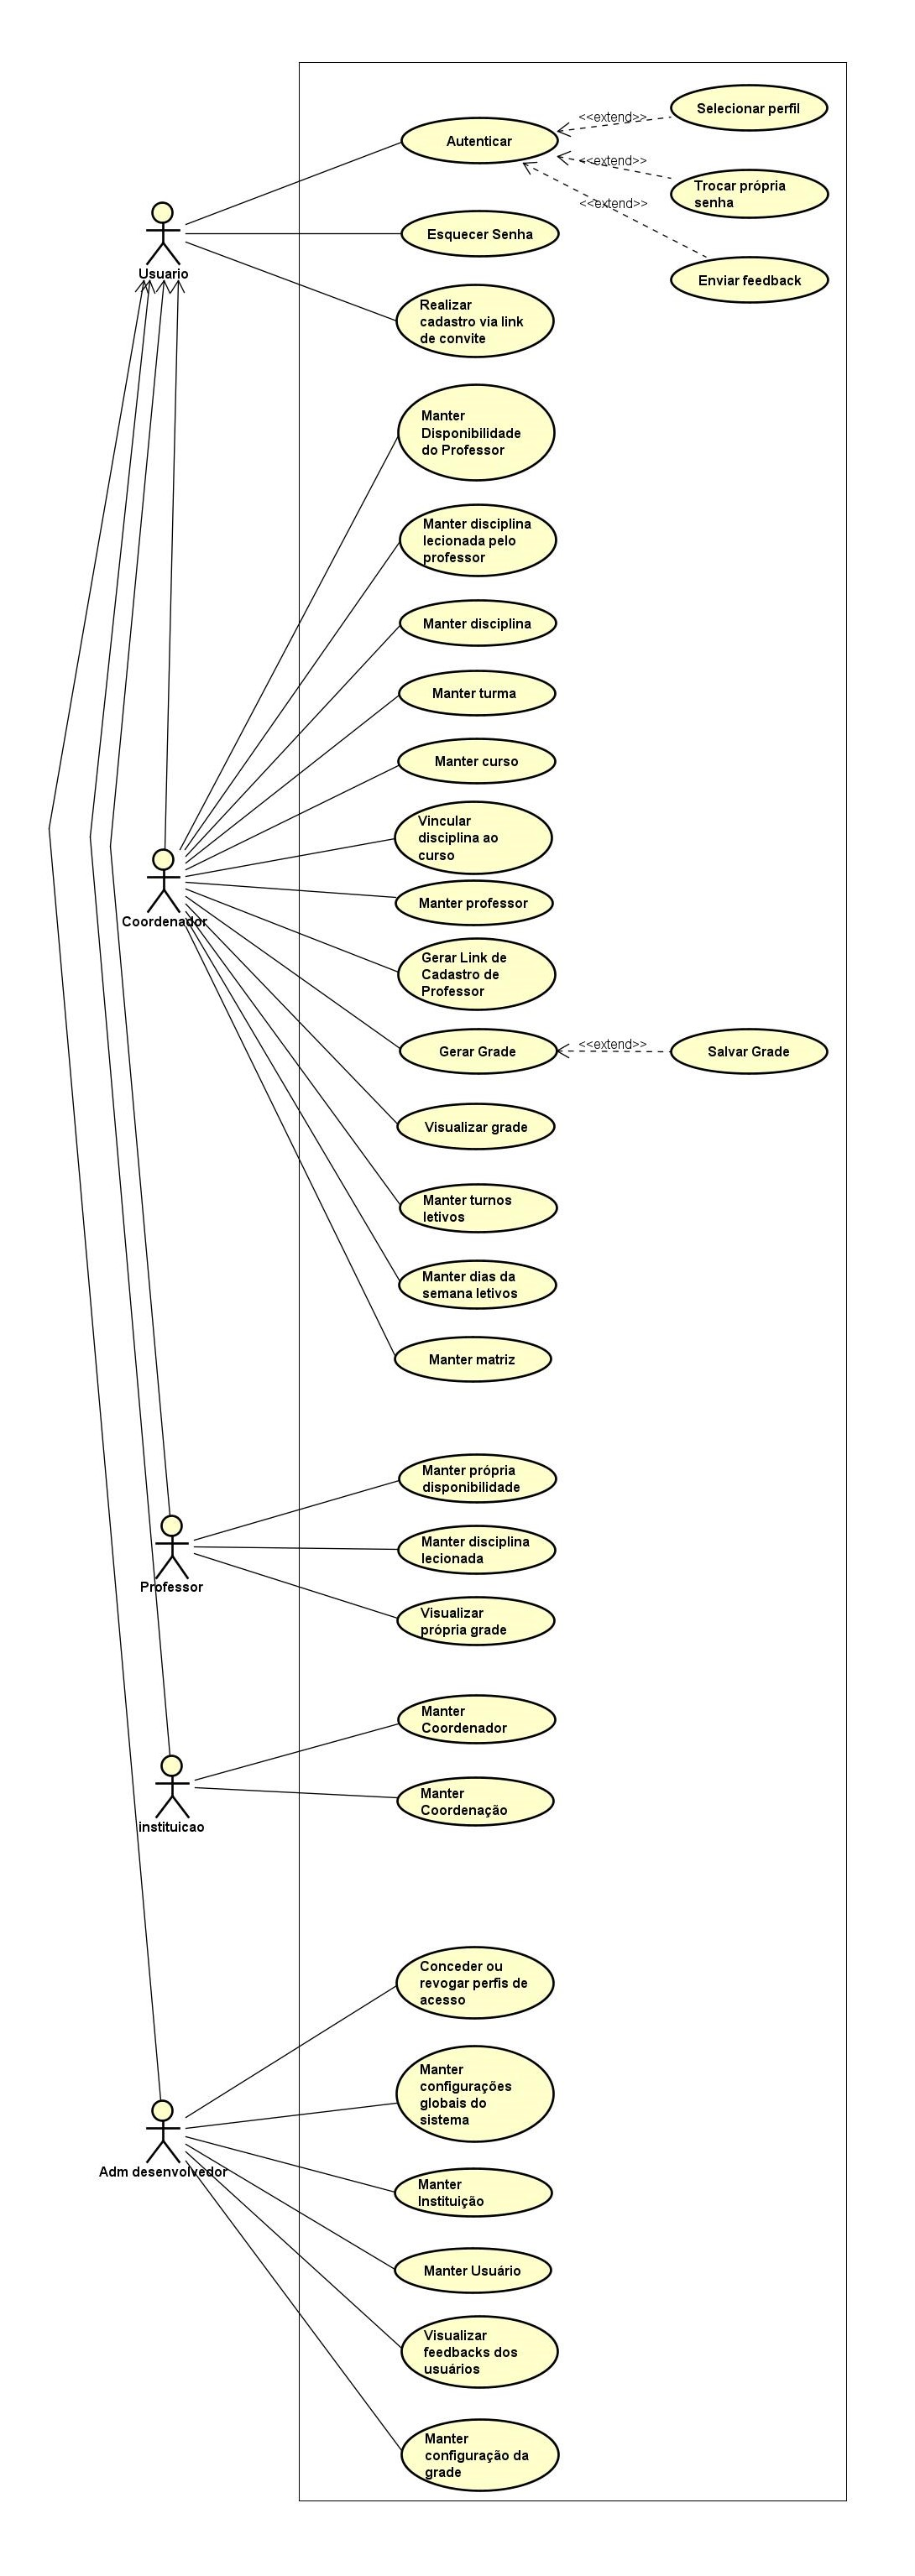
\includegraphics[width=\textwidth,height=0.86\textheight,keepaspectratio]{figuras/Figura_9_Diagrama de casos de uso.jpg}
\fonteautores
\end{figure}

\clearpage

\subsection{Descrição dos Casos de Uso}
\label{subsec:4.2.3}

Para eliminar ambiguidades inerentes à representação gráfica, os casos de uso foram detalhados textualmente seguindo o modelo de especificação padrão, com descrição, ator, pré-condição, pós-condição e fluxo principal de interação. Os Quadros de UC01 a UC33 apresentam a especificação completa de cada caso de uso do sistema.

% Tabela 3
\vspace{\baselineskip}

\Needspace{0.48\textheight}
\begin{longtable}{|L{4.5cm}|L{10.5cm}|}
\caption{Especificação do Caso de Uso: UC01 -- Autenticar} \\
\hline
\textbf{Nome do caso de uso} & \textbf{UC01 -- Autenticar} \\
\hline
\endfirsthead
\hline
\textbf{Nome do caso de uso} & \textbf{UC01 -- Autenticar} \\
\hline
\endhead
Descrição       & Permite que o usuário acesse o sistema de forma segura. \\
\hline
Ator            & Usuário \\
\hline
Pré-condição    & O usuário deve possuir um cadastro válido. \\
\hline
Pós-condição    & O usuário é logado no sistema e o token JWT é injetado. \\
\hline
Fluxo Principal & Ação do Ator: Informa login e senha e clica em entrar. Ação do Sistema: Valida credenciais no banco, gera o token de acesso e redireciona o usuário. \\
\hline
\end{longtable}

\fonteautores

% Tabela 4
\vspace{\baselineskip}

\Needspace{0.48\textheight}
\begin{longtable}{|L{4.5cm}|L{10.5cm}|}
\caption{Especificação do Caso de Uso: UC02 -- Selecionar/Trocar Perfil} \\
\hline
\textbf{Nome do caso de uso} & \textbf{UC02 -- Selecionar/Trocar Perfil} \\
\hline
\endfirsthead
\hline
\textbf{Nome do caso de uso} & \textbf{UC02 -- Selecionar/Trocar Perfil} \\
\hline
\endhead
Descrição       & Permite alterar o papel ativo na sessão (ex: trocar a visão de Professor para Coordenador). \\
\hline
Ator            & Usuário (Autenticado) \\
\hline
Pré-condição    & O usuário deve possuir múltiplos vínculos de perfis ativos. \\
\hline
Pós-condição    & O sistema reemite o token JWT com as permissões do novo perfil selecionado. \\
\hline
Fluxo Principal & Ação do Ator: Seleciona um novo perfil na interface e confirma. Ação do Sistema: Invalida o contexto anterior, emite novo token JWT e recarrega a página. \\
\hline
\end{longtable}

\fonteautores

% Tabela 5
\vspace{\baselineskip}

\Needspace{0.48\textheight}
\begin{longtable}{|L{4.5cm}|L{10.5cm}|}
\caption{Especificação do Caso de Uso: UC03 -- Trocar Própria Senha} \\
\hline
\textbf{Nome do caso de uso} & \textbf{UC03 -- Trocar Própria Senha} \\
\hline
\endfirsthead
\hline
\textbf{Nome do caso de uso} & \textbf{UC03 -- Trocar Própria Senha} \\
\hline
\endhead
Descrição       & Permite que o usuário altere sua senha por motivos de segurança. \\
\hline
Ator            & Usuário (Autenticado) \\
\hline
Pré-condição    & O usuário deve estar logado e saber sua senha atual. \\
\hline
Pós-condição    & A senha atual é substituída pela nova senha criptografada. \\
\hline
Fluxo Principal & Ação do Ator: Informa a senha atual e a nova senha desejada. Ação do Sistema: Valida a senha atual e criptografa e salva a nova. \\
\hline
\end{longtable}

\fonteautores

% Tabela 6
\vspace{\baselineskip}

\Needspace{0.48\textheight}
\begin{longtable}{|L{4.5cm}|L{10.5cm}|}
\caption{Especificação do Caso de Uso: UC04 -- Enviar Feedback} \\
\hline
\textbf{Nome do caso de uso} & \textbf{UC04 -- Enviar Feedback} \\
\hline
\endfirsthead
\hline
\textbf{Nome do caso de uso} & \textbf{UC04 -- Enviar Feedback} \\
\hline
\endhead
Descrição       & Enviar sugestões ou reportar bugs do sistema para os administradores. \\
\hline
Ator            & Usuário (Autenticado) \\
\hline
Pré-condição    & Estar logado no sistema. \\
\hline
Pós-condição    & O feedback é registrado na base atrelado ao usuário remetente. \\
\hline
Fluxo Principal & Ação do Ator: Seleciona a categoria, digita a mensagem e envia. Ação do Sistema: Salva o feedback no banco de dados. \\
\hline
\end{longtable}

\fonteautores

% Tabela 7
\vspace{\baselineskip}

\Needspace{0.48\textheight}
\begin{longtable}{|L{4.5cm}|L{10.5cm}|}
\caption{Especificação do Caso de Uso: UC05 -- Esquecer Senha} \\
\hline
\textbf{Nome do caso de uso} & \textbf{UC05 -- Esquecer Senha} \\
\hline
\endfirsthead
\hline
\textbf{Nome do caso de uso} & \textbf{UC05 -- Esquecer Senha} \\
\hline
\endhead
Descrição       & Permite ao usuário recuperar o acesso através de um link enviado por e-mail. \\
\hline
Ator            & Usuário \\
\hline
Pré-condição    & O usuário não consegue logar, mas possui acesso ao seu e-mail cadastrado. \\
\hline
Pós-condição    & Uma nova senha é cadastrada para o usuário. \\
\hline
Fluxo Principal & Ação do Ator: Solicita recuperação informando e-mail. Acessa o link e digita a nova senha. Ação do Sistema: Envia o e-mail com token. Valida o token e atualiza a senha no banco. \\
\hline
\end{longtable}

\fonteautores

% Tabela 8
\vspace{\baselineskip}

\Needspace{0.48\textheight}
\begin{longtable}{|L{4.5cm}|L{10.5cm}|}
\caption{Especificação do Caso de Uso: UC06 -- Realizar Cadastro via Link de Convite} \\
\hline
\textbf{Nome do caso de uso} & \textbf{UC06 -- Realizar Cadastro via Link de Convite} \\
\hline
\endfirsthead
\hline
\textbf{Nome do caso de uso} & \textbf{UC06 -- Realizar Cadastro via Link de Convite} \\
\hline
\endhead
Descrição       & Cadastro facilitado onde o professor já entra vinculado à faculdade. \\
\hline
Ator            & Usuário (Visitante/Professor) \\
\hline
Pré-condição    & Possuir um link/token de convite válido gerado por um coordenador. \\
\hline
Pós-condição    & Conta criada já com o perfil de Professor vinculado à instituição de origem do link. \\
\hline
Fluxo Principal & Ação do Ator: Acessa o link e preenche a senha e dados faltantes. Ação do Sistema: Valida o token do link, cria o usuário, atribui o perfil ACESSO\_PROFESSOR e expira o link. \\
\hline
\end{longtable}

\fonteautores

% Tabela 9
\vspace{\baselineskip}

\Needspace{0.48\textheight}
\begin{longtable}{|L{4.5cm}|L{10.5cm}|}
\caption{Especificação do Caso de Uso: UC07 -- Manter Disponibilidade do Professor} \\
\hline
\textbf{Nome do caso de uso} & \textbf{UC07 -- Manter Disponibilidade do Professor} \\
\hline
\endfirsthead
\hline
\textbf{Nome do caso de uso} & \textbf{UC07 -- Manter Disponibilidade do Professor} \\
\hline
\endhead
Descrição       & Permite ao coordenador visualizar e, se necessário, intervir na disponibilidade de tempo informada pelos professores. \\
\hline
Ator            & Coordenador \\
\hline
Pré-condição    & Professores devem possuir cadastro e vínculos na instituição. \\
\hline
Pós-condição    & A malha de disponibilidade dos professores fica pronta para o algoritmo. \\
\hline
Fluxo Principal & Ação do Ator: Consulta ou ajusta os dias/horários livres de um professor. Ação do Sistema: Salva a entidade Disponibilidade. \\
\hline
\end{longtable}

\fonteautores

% Tabela 10
\vspace{\baselineskip}

\Needspace{0.48\textheight}
\begin{longtable}{|L{4.5cm}|L{10.5cm}|}
\caption{Especificação do Caso de Uso: UC08 -- Manter Disciplina Lecionada pelo Professor} \\
\hline
\textbf{Nome do caso de uso} & \textbf{UC08 -- Manter Disciplina Lecionada pelo Professor} \\
\hline
\endfirsthead
\hline
\textbf{Nome do caso de uso} & \textbf{UC08 -- Manter Disciplina Lecionada pelo Professor} \\
\hline
\endhead
Descrição       & Permite ao coordenador gerenciar a equipe de professores e o que eles podem lecionar. \\
\hline
Ator            & Coordenador \\
\hline
Pré-condição    & Professores devem estar cadastrados na instituição. \\
\hline
Pós-condição    & Professor é mantido e vínculos com disciplinas são atualizados. \\
\hline
Fluxo Principal & Ação do Ator: Seleciona um professor e marca as disciplinas nas quais ele tem domínio. Ação do Sistema: Salva os registros na entidade UsuarioDisciplina. \\
\hline
\end{longtable}

\fonteautores

% Tabela 11
\vspace{\baselineskip}

\Needspace{0.48\textheight}
\begin{longtable}{|L{4.5cm}|L{10.5cm}|}
\caption{Especificação do Caso de Uso: UC09 -- Manter Disciplina} \\
\hline
\textbf{Nome do caso de uso} & \textbf{UC09 -- Manter Disciplina} \\
\hline
\endfirsthead
\hline
\textbf{Nome do caso de uso} & \textbf{UC09 -- Manter Disciplina} \\
\hline
\endhead
Descrição       & Permite gerenciar o catálogo global de disciplinas da coordenação. \\
\hline
Ator            & Coordenador \\
\hline
Pré-condição    & Estar logado como Coordenador. \\
\hline
Pós-condição    & A disciplina passa a existir no catálogo. \\
\hline
Fluxo Principal & Ação do Ator: Insere nome e carga horária da disciplina. Ação do Sistema: Persiste a disciplina no banco. \\
\hline
\end{longtable}

\fonteautores

% Tabela 12
\vspace{\baselineskip}

\Needspace{0.48\textheight}
\begin{longtable}{|L{4.5cm}|L{10.5cm}|}
\caption{Especificação do Caso de Uso: UC10 -- Manter Turma} \\
\hline
\textbf{Nome do caso de uso} & \textbf{UC10 -- Manter Turma} \\
\hline
\endfirsthead
\hline
\textbf{Nome do caso de uso} & \textbf{UC10 -- Manter Turma} \\
\hline
\endhead
Descrição       & Permite criar turmas de um curso para um determinado semestre/ano. \\
\hline
Ator            & Coordenador \\
\hline
Pré-condição    & Curso e Turno devem estar cadastrados. \\
\hline
Pós-condição    & Turma é instanciada e pronta para receber alunos/matrizes. \\
\hline
Fluxo Principal & Ação do Ator: Informa nome, curso, turno, semestre e ano. Ação do Sistema: Salva a entidade Turma vinculada à coordenação. \\
\hline
\end{longtable}

\fonteautores

% Tabela 13
\vspace{\baselineskip}

\Needspace{0.48\textheight}
\begin{longtable}{|L{4.5cm}|L{10.5cm}|}
\caption{Especificação do Caso de Uso: UC11 -- Manter Curso} \\
\hline
\textbf{Nome do caso de uso} & \textbf{UC11 -- Manter Curso} \\
\hline
\endfirsthead
\hline
\textbf{Nome do caso de uso} & \textbf{UC11 -- Manter Curso} \\
\hline
\endhead
Descrição       & Permite gerenciar os cursos oferecidos pela coordenação. \\
\hline
Ator            & Coordenador \\
\hline
Pré-condição    & Estar logado com o perfil de Coordenador. \\
\hline
Pós-condição    & Curso é criado, alterado ou removido logicamente. \\
\hline
Fluxo Principal & Ação do Ator: Preenche os dados do curso e solicita salvar. Ação do Sistema: Valida os dados e salva o curso atrelado à instituição/coordenação. \\
\hline
\end{longtable}

\fonteautores

% Tabela 14
\vspace{\baselineskip}

\Needspace{0.48\textheight}
\begin{longtable}{|L{4.5cm}|L{10.5cm}|}
\caption{Especificação do Caso de Uso: UC12 -- Vincular Disciplina ao Curso} \\
\hline
\textbf{Nome do caso de uso} & \textbf{UC12 -- Vincular Disciplina ao Curso} \\
\hline
\endfirsthead
\hline
\textbf{Nome do caso de uso} & \textbf{UC12 -- Vincular Disciplina ao Curso} \\
\hline
\endhead
Descrição       & Permite definir quais disciplinas fazem parte do catálogo de um curso. \\
\hline
Ator            & Coordenador \\
\hline
Pré-condição    & Curso e Disciplina devem existir. \\
\hline
Pós-condição    & Criado o relacionamento na tabela DisciplinaCurso. \\
\hline
Fluxo Principal & Ação do Ator: Seleciona o curso e marca as disciplinas pertencentes a ele. Ação do Sistema: Salva os vínculos na tabela de junção. \\
\hline
\end{longtable}

\fonteautores

% Tabela 15
\vspace{\baselineskip}

\Needspace{0.48\textheight}
\begin{longtable}{|L{4.5cm}|L{10.5cm}|}
\caption{Especificação do Caso de Uso: UC13 -- Manter Professor} \\
\hline
\textbf{Nome do caso de uso} & \textbf{UC13 -- Manter Professor} \\
\hline
\endfirsthead
\hline
\textbf{Nome do caso de uso} & \textbf{UC13 -- Manter Professor} \\
\hline
\endhead
Descrição       & Permite gerenciar os dados cadastrais básicos dos professores da instituição. \\
\hline
Ator            & Coordenador \\
\hline
Pré-condição    & Ter permissão de Coordenador. \\
\hline
Pós-condição    & Dados do professor são atualizados/cadastrados. \\
\hline
Fluxo Principal & Ação do Ator: Altera informações do professor. Ação do Sistema: Atualiza o cadastro no banco. \\
\hline
\end{longtable}

\fonteautores

% Tabela 16
\vspace{\baselineskip}

\Needspace{0.48\textheight}
\begin{longtable}{|L{4.5cm}|L{10.5cm}|}
\caption{Especificação do Caso de Uso: UC14 -- Gerar Link de Cadastro de Professor} \\
\hline
\textbf{Nome do caso de uso} & \textbf{UC14 -- Gerar Link de Cadastro de Professor} \\
\hline
\endfirsthead
\hline
\textbf{Nome do caso de uso} & \textbf{UC14 -- Gerar Link de Cadastro de Professor} \\
\hline
\endhead
Descrição       & Gera uma URL temporária criptografada para enviar a novos professores. \\
\hline
Ator            & Coordenador \\
\hline
Pré-condição    & Estar logado como coordenador da instituição. \\
\hline
Pós-condição    & Um link com token é gerado e retornado na tela. \\
\hline
Fluxo Principal & Ação do Ator: Clica no botão de gerar convite. Ação do Sistema: Cria um token seguro na entidade Link e exibe a URL. \\
\hline
\end{longtable}

\fonteautores

% Tabela 17
\vspace{\baselineskip}

\Needspace{0.48\textheight}
\begin{longtable}{|L{4.5cm}|L{10.5cm}|}
\caption{Especificação do Caso de Uso: UC15 -- Validar Usuários Cadastrados via Link} \\
\hline
\textbf{Nome do caso de uso} & \textbf{UC15 -- Validar Usuários Cadastrados via Link} \\
\hline
\endfirsthead
\hline
\textbf{Nome do caso de uso} & \textbf{UC15 -- Validar Usuários Cadastrados via Link} \\
\hline
\endhead
Descrição       & Permite ao coordenador aprovar ou rejeitar o acesso de professores que se cadastraram via link. \\
\hline
Ator            & Coordenador \\
\hline
Pré-condição    & Um professor deve ter concluído o cadastro através do link gerado. \\
\hline
Pós-condição    & O acesso do usuário é ativado ou desativado no sistema. \\
\hline
Fluxo Principal & Ação do Ator: Visualiza a lista de novos cadastros e altera o status para ativo ou inativo. Ação do Sistema: Atualiza a permissão de acesso do usuário no banco. \\
\hline
\end{longtable}

\fonteautores

% Tabela 18
\vspace{\baselineskip}

\Needspace{0.48\textheight}
\begin{longtable}{|L{4.5cm}|L{10.5cm}|}
\caption{Especificação do Caso de Uso: UC16 -- Gerar Grade} \\
\hline
\textbf{Nome do caso de uso} & \textbf{UC16 -- Gerar Grade} \\
\hline
\endfirsthead
\hline
\textbf{Nome do caso de uso} & \textbf{UC16 -- Gerar Grade} \\
\hline
\endhead
Descrição       & Aciona o algoritmo para montar o horário das turmas automaticamente. \\
\hline
Ator            & Coordenador \\
\hline
Pré-condição    & Turmas, professores, disciplinas (matrizes) e disponibilidades devem estar cadastradas. \\
\hline
Pós-condição    & Uma nova grade sugerida é retornada pelos microservices. \\
\hline
Fluxo Principal & Ação do Ator: Informa semestre/ano e clica em Gerar. Ação do Sistema: Envia os dados para os microservices (Sunny/Morpheus) e retorna a grade. \\
\hline
\end{longtable}

\fonteautores

% Tabela 19
\vspace{\baselineskip}

\Needspace{0.48\textheight}
\begin{longtable}{|L{4.5cm}|L{10.5cm}|}
\caption{Especificação do Caso de Uso: UC17 -- Salvar Grade} \\
\hline
\textbf{Nome do caso de uso} & \textbf{UC17 -- Salvar Grade} \\
\hline
\endfirsthead
\hline
\textbf{Nome do caso de uso} & \textbf{UC17 -- Salvar Grade} \\
\hline
\endhead
Descrição       & Efetiva a grade gerada ou manipulada manualmente no banco de dados. \\
\hline
Ator            & Coordenador \\
\hline
Pré-condição    & Uma grade válida deve estar em tela (Gerar Grade). \\
\hline
Pós-condição    & As alocações são persistidas e grades anteriores são arquivadas. \\
\hline
Fluxo Principal & Ação do Ator: Confirma as alocações e clica em Salvar. Ação do Sistema: Salva a nova entidade Grade e suas Alocacoes. \\
\hline
\end{longtable}

\fonteautores

% Tabela 20
\vspace{\baselineskip}

\Needspace{0.48\textheight}
\begin{longtable}{|L{4.5cm}|L{10.5cm}|}
\caption{Especificação do Caso de Uso: UC18 -- Visualizar Grade} \\
\hline
\textbf{Nome do caso de uso} & \textbf{UC18 -- Visualizar Grade} \\
\hline
\endfirsthead
\hline
\textbf{Nome do caso de uso} & \textbf{UC18 -- Visualizar Grade} \\
\hline
\endhead
Descrição       & Consultar a grade atualizada do semestre em vigor ou o histórico. \\
\hline
Ator            & Coordenador \\
\hline
Pré-condição    & A grade deve ter sido gerada e salva previamente. \\
\hline
Pós-condição    & O cronograma é exibido em formato de calendário/tabela. \\
\hline
Fluxo Principal & Ação do Ator: Seleciona o semestre/ano desejado. Ação do Sistema: Busca a Grade ativa e a exibe renderizada por turmas. \\
\hline
\end{longtable}

\fonteautores

% Tabela 21
\vspace{\baselineskip}

\Needspace{0.48\textheight}
\begin{longtable}{|L{4.5cm}|L{10.5cm}|}
\caption{Especificação do Caso de Uso: UC19 -- Manter Turnos Letivos} \\
\hline
\textbf{Nome do caso de uso} & \textbf{UC19 -- Manter Turnos Letivos} \\
\hline
\endfirsthead
\hline
\textbf{Nome do caso de uso} & \textbf{UC19 -- Manter Turnos Letivos} \\
\hline
\endhead
Descrição       & Gerenciar os turnos disponíveis (Matutino, Vespertino, Noturno). \\
\hline
Ator            & Coordenador \\
\hline
Pré-condição    & Estar logado como Coordenador. \\
\hline
Pós-condição    & Turnos são atualizados para uso. \\
\hline
Fluxo Principal & Ação do Ator: Adiciona ou altera nomes/horários de turnos. Ação do Sistema: Atualiza a entidade Turno. \\
\hline
\end{longtable}

\fonteautores

% Tabela 22
\vspace{\baselineskip}

\Needspace{0.48\textheight}
\begin{longtable}{|L{4.5cm}|L{10.5cm}|}
\caption{Especificação do Caso de Uso: UC20 -- Manter Dias da Semana Letivos} \\
\hline
\textbf{Nome do caso de uso} & \textbf{UC20 -- Manter Dias da Semana Letivos} \\
\hline
\endfirsthead
\hline
\textbf{Nome do caso de uso} & \textbf{UC20 -- Manter Dias da Semana Letivos} \\
\hline
\endhead
Descrição       & Gerenciar quais dias da semana ocorrem aulas na coordenação. \\
\hline
Ator            & Coordenador \\
\hline
Pré-condição    & Estar logado como Coordenador. \\
\hline
Pós-condição    & Dias úteis são atualizados para uso. \\
\hline
Fluxo Principal & Ação do Ator: Adiciona ou altera dias da semana. Ação do Sistema: Atualiza a entidade DiaSemana. \\
\hline
\end{longtable}

\fonteautores

% Tabela 23
\vspace{\baselineskip}

\Needspace{0.48\textheight}
\begin{longtable}{|L{4.5cm}|L{10.5cm}|}
\caption{Especificação do Caso de Uso: UC21 -- Manter Matriz} \\
\hline
\textbf{Nome do caso de uso} & \textbf{UC21 -- Manter Matriz} \\
\hline
\endfirsthead
\hline
\textbf{Nome do caso de uso} & \textbf{UC21 -- Manter Matriz} \\
\hline
\endhead
Descrição       & Permite vincular as disciplinas que uma turma específica terá em um determinado semestre. \\
\hline
Ator            & Coordenador \\
\hline
Pré-condição    & A Turma e as Disciplinas devem estar cadastradas. \\
\hline
Pós-condição    & O vínculo (Matriz) é salvo, servindo de base para o algoritmo gerar a grade. \\
\hline
Fluxo Principal & Ação do Ator: Seleciona uma turma e escolhe as disciplinas que comporão o semestre dela. Ação do Sistema: Salva os registros na entidade Matriz. \\
\hline
\end{longtable}

\fonteautores

% Tabela 24
\vspace{\baselineskip}

\Needspace{0.48\textheight}
\begin{longtable}{|L{4.5cm}|L{10.5cm}|}
\caption{Especificação do Caso de Uso: UC22 -- Manter Própria Disponibilidade} \\
\hline
\textbf{Nome do caso de uso} & \textbf{UC22 -- Manter Própria Disponibilidade} \\
\hline
\endfirsthead
\hline
\textbf{Nome do caso de uso} & \textbf{UC22 -- Manter Própria Disponibilidade} \\
\hline
\endhead
Descrição       & Informar à coordenação quais dias e turnos o professor tem horário livre para dar aula. \\
\hline
Ator            & Professor \\
\hline
Pré-condição    & Estar logado com o perfil de Professor. \\
\hline
Pós-condição    & A disponibilidade do semestre é salva no banco. \\
\hline
Fluxo Principal & Ação do Ator: Seleciona ano/semestre e marca em uma grade os horários livres. Ação do Sistema: Verifica duplicidades e salva as opções em Disponibilidade. \\
\hline
\end{longtable}

\fonteautores

% Tabela 25
\vspace{\baselineskip}

\Needspace{0.48\textheight}
\begin{longtable}{|L{4.5cm}|L{10.5cm}|}
\caption{Especificação do Caso de Uso: UC23 -- Manter Disciplina Lecionada} \\
\hline
\textbf{Nome do caso de uso} & \textbf{UC23 -- Manter Disciplina Lecionada} \\
\hline
\endfirsthead
\hline
\textbf{Nome do caso de uso} & \textbf{UC23 -- Manter Disciplina Lecionada} \\
\hline
\endhead
Descrição       & Visualizar quais disciplinas o coordenador vinculou ao seu perfil, ou solicitar alterações. \\
\hline
Ator            & Professor \\
\hline
Pré-condição    & Ter perfil de professor. \\
\hline
Pós-condição    & Exibe a lista de disciplinas atribuídas a ele. \\
\hline
Fluxo Principal & Ação do Ator: Acessa a tela de currículo/disciplinas. Ação do Sistema: Busca e lista as disciplinas da entidade UsuarioDisciplina. \\
\hline
\end{longtable}

\fonteautores

% Tabela 26
\vspace{\baselineskip}

\Needspace{0.48\textheight}
\begin{longtable}{|L{4.5cm}|L{10.5cm}|}
\caption{Especificação do Caso de Uso: UC24 -- Visualizar Própria Grade} \\
\hline
\textbf{Nome do caso de uso} & \textbf{UC24 -- Visualizar Própria Grade} \\
\hline
\endfirsthead
\hline
\textbf{Nome do caso de uso} & \textbf{UC24 -- Visualizar Própria Grade} \\
\hline
\endhead
Descrição       & Consultar seu próprio cronograma de aulas na semana. \\
\hline
Ator            & Professor \\
\hline
Pré-condição    & A grade do semestre deve estar finalizada e salva pelo coordenador. \\
\hline
Pós-condição    & Exibe apenas as alocações que o envolvem. \\
\hline
Fluxo Principal & Ação do Ator: Acessa a visualização de horários. Ação do Sistema: Filtra a Grade ativa buscando apenas alocações vinculadas ao seu ID e exibe. \\
\hline
\end{longtable}

\fonteautores

% Tabela 27
\vspace{\baselineskip}

\Needspace{0.48\textheight}
\begin{longtable}{|L{4.5cm}|L{10.5cm}|}
\caption{Especificação do Caso de Uso: UC25 -- Manter Coordenador} \\
\hline
\textbf{Nome do caso de uso} & \textbf{UC25 -- Manter Coordenador} \\
\hline
\endfirsthead
\hline
\textbf{Nome do caso de uso} & \textbf{UC25 -- Manter Coordenador} \\
\hline
\endhead
Descrição       & Atribuir ou remover o cargo de coordenação a usuários. \\
\hline
Ator            & Adm Instituição \\
\hline
Pré-condição    & O usuário a ser promovido já deve estar cadastrado. \\
\hline
Pós-condição    & O usuário ganha o perfil ACESSO\_COORDENADOR. \\
\hline
Fluxo Principal & Ação do Ator: Seleciona um usuário e o vincula a uma Coordenação específica. Ação do Sistema: Cria o vínculo UsuarioPerfil e CoordenacaoVinculo. \\
\hline
\end{longtable}

\fonteautores

% Tabela 28
\vspace{\baselineskip}

\Needspace{0.48\textheight}
\begin{longtable}{|L{4.5cm}|L{10.5cm}|}
\caption{Especificação do Caso de Uso: UC26 -- Manter Coordenação} \\
\hline
\textbf{Nome do caso de uso} & \textbf{UC26 -- Manter Coordenação} \\
\hline
\endfirsthead
\hline
\textbf{Nome do caso de uso} & \textbf{UC26 -- Manter Coordenação} \\
\hline
\endhead
Descrição       & Gerenciar quais polos ou departamentos de coordenação existem na faculdade. \\
\hline
Ator            & Adm Instituição \\
\hline
Pré-condição    & Ter permissão ACESSO\_ADMIN\_INSTITUICAO. \\
\hline
Pós-condição    & Coordenações são adicionadas ou editadas na Instituição. \\
\hline
Fluxo Principal & Ação do Ator: Informa o nome do departamento e salva. Ação do Sistema: Salva a entidade Coordenacao vinculada à Instituicao. \\
\hline
\end{longtable}

\fonteautores

% Tabela 29
\vspace{\baselineskip}

\Needspace{0.48\textheight}
\begin{longtable}{|L{4.5cm}|L{10.5cm}|}
\caption{Especificação do Caso de Uso: UC27 -- Conceder ou Revogar Perfis de Acesso} \\
\hline
\textbf{Nome do caso de uso} & \textbf{UC27 -- Conceder ou Revogar Perfis de Acesso} \\
\hline
\endfirsthead
\hline
\textbf{Nome do caso de uso} & \textbf{UC27 -- Conceder ou Revogar Perfis de Acesso} \\
\hline
\endhead
Descrição       & Gerenciar dinamicamente quais perfis (Professor, etc.) os usuários da instituição possuem. \\
\hline
Ator            & Adm Instituição \\
\hline
Pré-condição    & Ter permissão ACESSO\_ADMIN\_INSTITUICAO. \\
\hline
Pós-condição    & Perfis são atualizados no banco para o usuário selecionado. \\
\hline
Fluxo Principal & Ação do Ator: Seleciona o usuário e adiciona ou retira permissões. Ação do Sistema: Atualiza a tabela de junção UsuarioPerfil. \\
\hline
\end{longtable}

\fonteautores

% Tabela 30
\vspace{\baselineskip}

\Needspace{0.48\textheight}
\begin{longtable}{|L{4.5cm}|L{10.5cm}|}
\caption{Especificação do Caso de Uso: UC28 -- Manter Configurações da Faculdade} \\
\hline
\textbf{Nome do caso de uso} & \textbf{UC28 -- Manter Configurações da Faculdade} \\
\hline
\endfirsthead
\hline
\textbf{Nome do caso de uso} & \textbf{UC28 -- Manter Configurações da Faculdade} \\
\hline
\endhead
Descrição       & Alterar parâmetros locais da faculdade, como restrições de horários institucionais. \\
\hline
Ator            & Adm Instituição \\
\hline
Pré-condição    & Ter permissão ACESSO\_ADMIN\_INSTITUICAO. \\
\hline
Pós-condição    & A entidade ConfigFaculdade é atualizada. \\
\hline
Fluxo Principal & Ação do Ator: Altera parâmetros no painel de configurações. Ação do Sistema: Persiste as opções no banco. \\
\hline
\end{longtable}

\fonteautores

% Tabela 31
\vspace{\baselineskip}

\Needspace{0.48\textheight}
\begin{longtable}{|L{4.5cm}|L{10.5cm}|}
\caption{Especificação do Caso de Uso: UC29 -- Manter Configurações Globais do Sistema} \\
\hline
\textbf{Nome do caso de uso} & \textbf{UC29 -- Manter Configurações Globais do Sistema} \\
\hline
\endfirsthead
\hline
\textbf{Nome do caso de uso} & \textbf{UC29 -- Manter Configurações Globais do Sistema} \\
\hline
\endhead
Descrição       & Alterar hiperparâmetros matemáticos dos microservices e variáveis do sistema (Modo Manutenção). \\
\hline
Ator            & Adm Desenvolvedor \\
\hline
Pré-condição    & Estar autenticado como ACESSO\_ADMIN. \\
\hline
Pós-condição    & Variáveis em banco e em memória de Cache são atualizadas em tempo real. \\
\hline
Fluxo Principal & Ação do Ator: Acessa o painel Dinâmico e altera parâmetros (tamanho da população, número de gerações, taxa de \textit{crossover}, taxa de mutação, taxa de elitismo, tamanho do torneio, penalidade de conflito, pontuação base, bônus de diversidade). Ação do Sistema: Salva na entidade ConfigSistema e limpa o cache. \\
\hline
\end{longtable}

\fonteautores

% Tabela 32
\vspace{\baselineskip}

\Needspace{0.48\textheight}
\begin{longtable}{|L{4.5cm}|L{10.5cm}|}
\caption{Especificação do Caso de Uso: UC30 -- Manter Instituição} \\
\hline
\textbf{Nome do caso de uso} & \textbf{UC30 -- Manter Instituição} \\
\hline
\endfirsthead
\hline
\textbf{Nome do caso de uso} & \textbf{UC30 -- Manter Instituição} \\
\hline
\endhead
Descrição       & Cadastrar e gerenciar novas Universidades ou Faculdades (clientes) no sistema. \\
\hline
Ator            & Adm Desenvolvedor \\
\hline
Pré-condição    & Estar autenticado como ACESSO\_ADMIN. \\
\hline
Pós-condição    & Uma nova Instituição passa a existir e poder comportar usuários. \\
\hline
Fluxo Principal & Ação do Ator: Insere nome, dados da Instituição. Ação do Sistema: Salva a entidade Instituicao. \\
\hline
\end{longtable}

\fonteautores

% Tabela 33
\vspace{\baselineskip}

\Needspace{0.48\textheight}
\begin{longtable}{|L{4.5cm}|L{10.5cm}|}
\caption{Especificação do Caso de Uso: UC31 -- Manter Usuário} \\
\hline
\textbf{Nome do caso de uso} & \textbf{UC31 -- Manter Usuário} \\
\hline
\endfirsthead
\hline
\textbf{Nome do caso de uso} & \textbf{UC31 -- Manter Usuário} \\
\hline
\endhead
Descrição       & Gerenciamento global e absoluto de todos os usuários cadastrados. \\
\hline
Ator            & Adm Desenvolvedor \\
\hline
Pré-condição    & Estar autenticado como ACESSO\_ADMIN. \\
\hline
Pós-condição    & Contas podem ser suspensas, editadas ou removidas. \\
\hline
Fluxo Principal & Ação do Ator: Consulta a base completa de usuários e aplica edições. Ação do Sistema: Atualiza o registro do usuário na base. \\
\hline
\end{longtable}

\fonteautores

% Tabela 34
\vspace{\baselineskip}

\Needspace{0.48\textheight}
\begin{longtable}{|L{4.5cm}|L{10.5cm}|}
\caption{Especificação do Caso de Uso: UC32 -- Manter Perfis de Acesso do Sistema} \\
\hline
\textbf{Nome do caso de uso} & \textbf{UC32 -- Manter Perfis de Acesso do Sistema} \\
\hline
\endfirsthead
\hline
\textbf{Nome do caso de uso} & \textbf{UC32 -- Manter Perfis de Acesso do Sistema} \\
\hline
\endhead
Descrição       & Gerenciar os papéis fundamentais (Roles) e privilégios disponíveis no sistema. \\
\hline
Ator            & Adm Desenvolvedor \\
\hline
Pré-condição    & Estar autenticado como ACESSO\_ADMIN. \\
\hline
Pós-condição    & Permissões globais são alteradas. \\
\hline
Fluxo Principal & Ação do Ator: Edita perfis de acesso nativos. Ação do Sistema: Atualiza a entidade Perfil na base. \\
\hline
\end{longtable}

\fonteautores

% Tabela 35
\vspace{\baselineskip}

\Needspace{0.48\textheight}
\begin{longtable}{|L{4.5cm}|L{10.5cm}|}
\caption{Especificação do Caso de Uso: UC33 -- Visualizar Feedbacks dos Usuários} \\
\hline
\textbf{Nome do caso de uso} & \textbf{UC33 -- Visualizar Feedbacks dos Usuários} \\
\hline
\endfirsthead
\hline
\textbf{Nome do caso de uso} & \textbf{UC33 -- Visualizar Feedbacks dos Usuários} \\
\hline
\endhead
Descrição       & Ler relatórios de erros/sugestões enviados por usuários e gerenciar o fluxo de chamados. \\
\hline
Ator            & Adm Desenvolvedor \\
\hline
Pré-condição    & Estar autenticado como ACESSO\_ADMIN. \\
\hline
Pós-condição    & Feedback é lido/arquivado e ações tomadas. \\
\hline
Fluxo Principal & Ação do Ator: Acessa a caixa de feedback recebida. Ação do Sistema: Consulta e exibe as listagens de Feedback da base. \\
\hline
\end{longtable}

\fonteautores

% Chapter 5
